\documentclass[12pt]{amsart}
\usepackage[T1]{fontenc}
\usepackage[utf8]{inputenc}

\usepackage[top=1.95cm, bottom=1.95cm, left=2.35cm, right=2.35cm]{geometry}

\usepackage{hyperref}
\usepackage{enumitem}
\usepackage{tcolorbox}
\usepackage{float}
\usepackage{cleveref}
\usepackage{multicol}
\usepackage{fancyvrb}
\usepackage{amsmath}
\usepackage[french]{babel}
\usepackage[
    type={CC},
    modifier={by-nc-sa},
	version={4.0},
]{doclicense}

\newcommand\floor[1]{\left\lfloor #1 \right\rfloor}

\usepackage{lymath}


\newtheorem{fact}{Fait}[section]
\newtheorem{example}{Exemple}[section]
\newtheorem{remark}{Remarque}[section]
\newtheorem*{proof*}{Preuve}

\setlength\parindent{0pt}

\floatstyle{boxed} 
\restylefloat{figure}


\DeclareMathOperator{\taille}{\text{\normalfont\texttt{taille}}}

\newcommand\sqseq[2]{\fbox{$#1$}_{\,\,#2}}


\DefineVerbatimEnvironment{rawcode}%
	{Verbatim}%
	{tabsize=4,%
	 frame=lines, framerule=0.3mm, framesep=2.5mm}
	 
	 
	 
\begin{document}

\title{BROUILLON - Sommer les carrés des chiffres d'un naturel}
\author{Christophe BAL}
\date{6 Juin 2018 -- 16 Jan. 2019}

\maketitle

\begin{center}
	\itshape
	Document, avec son source \LaTeX, disponible sur la page
	
	\url{https://github.com/bc-writing/drafts}.
\end{center}


\bigskip


\begin{center}
	\hrule\vspace{.3em}
	{
		\fontsize{1.35em}{1em}\selectfont
		\textbf{Mentions \og légales \fg}
	}
			
	\vspace{0.45em}
	\doclicenseThis
	\hrule
\end{center}


\setcounter{tocdepth}{1}
\tableofcontents



\section{Faire une tête au carré à tous les entiers naturels}

Voici un procédé facile à faire à l'aide d'une calculatrice.


\medskip

\begin{tcolorbox}
	Considérons un entier naturel $n$.
	
	\begin{itemize}[label = \small\textbullet]
		\item Élevons chacun des chiffres de $n$ au carré.
		
		\item Additionnons tous ces carrés. Notons $n$ cette somme.
		
		\item Retournons au premier point.
	\end{itemize}

	On peut alors étudier ce processus qui peut être infini a priori.
\end{tcolorbox}

Voici deux exemples instructifs pour la suite.


\begin{example}
	Pour $n = 19$, nous obtenons :
	\begin{itemize}[label=\textbullet]
		\item $1^2 + 9^2 = 82$
		\item $8^2 + 2^2 = 68$
		\item $6^2 + 8^2 = 100$
		\item $1^2 + 0^2 + 0^2 = 1$ $\rightarrow$ Rien de nouveau à attendre.
	\end{itemize}
\end{example}


\begin{example}
	Pour $n = 1\,234\,567\,890$, après $1^2 + 2^2 + 3^2 + 4^2 + 5^2 + 6^2 + 7^2 + 8^2 + 9^2 + 0^2 = 285$ nous obtenons :
	\vspace{-.7em}
	\begin{multicols}{2}
		\begin{itemize}[label=\textbullet]
			\item $2^2 + 8^2 + 5^2 = 93$
			\item $9^2 + 3^2 = 90$
			\item $9^2 + 0^2 = 81$
			\item $8^2 + 1^2 = 65$
			\item $6^2 + 5^2 = 61$
			\item $6^2 + 1^2 = 37$
			\item $3^2 + 7^2 = 58$
		\end{itemize}
		\columnbreak
		\begin{itemize}[label=\textbullet]
			\item $5^2 + 8^2 = 89$
			\item $8^2 + 9^2 = 145$
			\item $1^2 + 4^2 + 5^2 = 42$
			\item $4^2 + 2^2 = 20$
			\item $2^2 + 0^2 = 4$
			\item $4^2 = 16$ 
			\item $1^2 + 6^2 = 37$ $\rightarrow$ Dèjà rencontré.
		\end{itemize}
	\end{multicols}
\end{example}

Dans le 1\ier{} cas, au bout d'un moment le procédé ne produit que des $1$. Ce sera par exemple le cas dès que l'on commence avec une puissance de $10$.
Quant au 2\ieme{} exemple, il montre que le mieux que l'on puisse espérer c'est que le procédé devienne périodique à partir d'un moment \emph{(on parle de phénomène ultimement périodique)}.


\medskip

On peut explorer le comportement de ce procédé sur plusieurs valeurs grâce à un programme. Voici un code possible non optimisé écrit en Python 3.7 qui prend un peu de temps pour vérifier que pour tous les naturels $n \in \ZintervalC{1}{10^6}$, le procédé devient ultimement périodique.

\begin{rawcode}
NMAX    = 10**6
MAXLOOP = 10**20

for n in range(1, NMAX + 1):
    nbloops = 0
    results = []

    while nbloops < MAXLOOP and n not in results:
        nbloops += 1
        results.append(n)
        n = sum(int(d)**2 for d in str(n))

    if n not in results:
        print(f"Test raté pour n = {n}.")

print("Tests finis.")
\end{rawcode}

\medskip

Une fois lancé, le code précédent affiche juste \verb+Tests finis+.
Il reste à voir ce qu'il se passe dans le cas général. La section qui suit démontre que pour tout naturel $n$, le procédé sera toujours ultimement périodique.




\section{Une preuve}\label{proof}

On introduit les notations suivantes.
\begin{itemize}[label = \textbullet]
	\item Pour un naturel $n$,
	$\displaystyle      n =  \left[ \, c_{d-1} c_{d-2} \cdots c_1 c_0 \, \right]_{10} 
	\stackrel{\text{def}}{=} \sum_{k=0}^{d-1} c_k 10^k$,
	avec $c_{d-1} \neq 0$, désigne l'écriture décimale propre de $n$.
	
	\item On pose enuite
	$\displaystyle sq(n) = \sum_{k=0}^{d-1} (c_k)^2$
	et
	$\taille(n) = d$ sera appelé \emph{\og taille de $n$ \fg}.


	\item Pour $(n \,; k) \in \NN^2$, on définit 
	$  \sqseq{n}{0} = n$
	et
	$  \sqseq{n}{k} = sq^k(n)
	\stackrel{\text{def}}{=} sq \,\circ sq \,\circ \cdots \,\circ sq(n)$ avec $(k-1)$ compositions si $k > 0$.
	
	
	\smallskip\noindent
	Autrement dit, nous avons
	$\sqseq{n}{0} = n$
	et
	$\sqseq{n}{k+1} = sq \left( \, \sqseq{n}{k} \right)$.


	\item Enfin on note
	$V_n = \geneset{ \, \sqseq{n}{k} \, | \, k \in \NN }$
	l'ensemble des valeurs prises par la suite $\left( \, \sqseq{n}{k} \right)_k$.
\end{itemize}



\bigskip

\begin{fact}
	$\forall n \in \NN$, $sq(n) \leqslant 81 d$ où $d = \taille(n)$.
\end{fact}

\begin{proof*}
	Si $n = \left[ \, c_{d-1} c_{d-2} \cdots c_1 c_0 \, \right]_{10}$
	alors 
	$\displaystyle sq(n) = \sum_{k=0}^{d-1} (c_k)^2 \leqslant \sum_{k=0}^{d-1} 9^2 = 81 d $.
\end{proof*}




\medskip

\begin{fact}\label{magicmajo}
	$\forall n \in \NN$, notant $d = \taille(n)$, nous avons les résultats suivants :
	
	\begin{enumerate}
		\item Si $d \geqslant 4$ alors $sq(n) < n$.
		
		\item Si $d \leqslant 3$ alors $sq(n) < 10^3$.
	\end{enumerate}
\end{fact}

\begin{proof*}
	Comme $n \geqslant 10^{d-1}$ et compte tenu du fait précédent, nous cherchons à comparer $10^{d-1}$ et $81d$.
	Pour cela, regardons ce qu'il se passe pour les premières valeurs de $d$.

	\smallskip
	\begin{center}
		\begin{tabular}{|r|c|c|c|c|c|}
			\hline
				$d$        & $1$  & $2$   & $3$   & $4$    & $5$        \\
			\hline
				$10^{d-1}$ & $1$  & $10$  & $100$ & $1000$ & $10\,000$  \\
			\hline
				$81d$      & $81$ & $162$ & $243$ & $324$  & $405$      \\
			\hline
		\end{tabular}
	\end{center}
	\smallskip
	
	Or lorsque $d \geqslant 2$ augmente de $1$, alors $81d$ augmente de $81$ tandis que $10^{d-1}$ augmente d'au moins $100$.
	Nous en déduisons que $n \geqslant 10^{d-1} > 81d \geqslant sq(n)$ , d'où $n > sq(n)$ , dès que $d \geqslant 4$.
	Ceci prouve le 1\ier{} point.
	Pour les fans de Nicolas B.
	\footnote{
		Alias Nicolas BOURBAKI.
	}, 
	voir la preuve \cpageref{magicmajo-proof} du fait \ref{magicmajo} qui traite le cas d'une puissance quelconque.


	\bigskip
	
	Le 2nd point pour $d \leqslant 3$ découle directement de $sq(999) = 243$.
\end{proof*}




\medskip

\begin{fact}
	$\forall n \in \NN$, l'ensemble $V_n$ est fini et donc la suite $\left( \, \sqseq{n}{k} \right)_{k \in \NN}$ est ultimement périodique, i.e. périodique à partir d'un certain rang.
\end{fact}

\begin{proof*}
	Le 2nd point dépend directement du 1er point via le principe des tiroirs et la définition récursive de la suite $\left( \, \sqseq{n}{k} \right)_k$.
	
	\medskip
	
	Pour le 1er point, pour $n \leqslant 999$, on a directement $V_n \subset \intervalC{0}{999}$,
	sinon il suffit de montrer que $V_n \subset \intervalC{0}{10^{\taille(n)}}$ pour $n \geqslant 10^4$ via une petite récurrence descendante finie.
\end{proof*}


\section{Coder - Étudier la \og période \fg{} d'un naturel}

Quand il ne se fige pas, le code suivant donne la \textit{\og période \fg} d'un naturel auquel on applique le procédé présenté dans la section \ref{conjecture}.

\begin{rawcode}
n     = 20181209
nmemo = n

results = []

while n not in results:
    results.append(n)
    n = sum(int(d)**2 for d in str(n))

print(f"{nmemo} a la période suivante :")
print(results[results.index(n):])

print()

before = results[:results.index(n)]

if before:
    print("Avant la 1ère période nous avons :")
    print(before)
else:
    print("On commence directement par la période.")
\end{rawcode}

\medskip

Le code précédent, où \verb+n = 20181209+, nous affiche :

\begin{rawcode}
20181209 a la période suivante :
[16, 37, 58, 89, 145, 42, 20, 4]

Avant la 1ère période nous avons :
[20181209, 155, 51, 26, 40]
\end{rawcode}


\medskip

\begin{figure}[t]
	\centering
	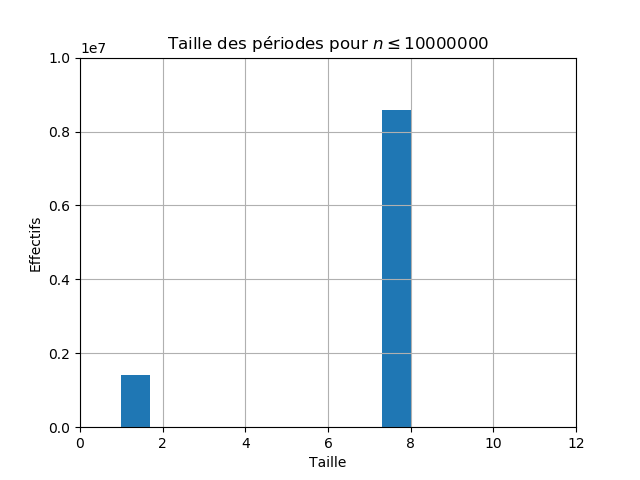
\includegraphics[scale=.9]{squares-int/periods.png}
  	\caption{Histogramme des tailles des périodes}
	\label{histogram}
\end{figure}



\medskip

Amusons-nous maintenant à représenter un histogramme des tailles des \og périodes \fg{}
À l'adresse \url{https://github.com/bc-writing/drafts}, dans le dossier \texttt{squares-int}, vous trouverez le fichier \texttt{squareint-sizeplots.py} qui été utilisé pour obtenir le graphique
\footnote{
	À la même adresse dans le dossier \texttt{squares-int} se trouve l'image \texttt{befores.png} qui est un histogramme des nombres de termes calculés avant l'apparition de la 1\iere{} \emph{\og période \fg{}}.
}.
Le traitement des données a été amélioré pour éviter de refaire des calculs déjà rencontrés \emph{(pour plus de précisions, se reporter aux commentaires du code)}.
Le résultat est donné dans la figure \ref{histogram} \cpageref{histogram}.



\medskip

Le graphique est frappant ! En effet, il semblerait que l'on ait soit des périodes de taille $1$, penser à $0$ et $1$, soit des périodes de taille $8$ comme pour $37 - 58 - 89 - 145 - 42 - 20 - 4 - 16$.
Magie ou coïncidence ? Les résultats de la section \ref{proof}, dont nous allons reprendre les notations, vont nous permettre de le savoir.
Tout d'abord,  d'après le fait \ref{magicmajo}, nous avons $\taille(sq(n)) < \taille(n)$ dès que $\taille(n) \geqslant 4$, donc la périodicité n'arrivera que lorsque $\taille\left( \, \sqseq{n}{k} \right) \leqslant 3$.
De plus, nous savons aussi que $\taille(sq(n)) \leqslant 3$ dès que $\taille(n) \leqslant 3$.
Tout ceci nous permet d'analyser brutalement via un programme ce qu'il se passe pour les périodes des naturels appartenant à $\ZintervalC{0}{999}$. Nous pouvons pour cela utiliser le code suivant, qui n'est absolument pas optimisé mais fait le travail immédiatement.


\newpage

\begin{rawcode}
nmax = 999

periodsfound = []

for n in range(nmax + 1):
    results = []

    while n not in results:
        results.append(n)
        n = sum(int(d)**2 for d in str(n))

    period = results[results.index(n):]

    if period not in periodsfound:
        periodsfound.append(period)

for oneperiod in periodsfound:
    print(oneperiod)
\end{rawcode}



\medskip

Le code précédent nous fournit toutes les périodes possibles.


\newpage

\begin{rawcode}
[0]
[1]
[4, 16, 37, 58, 89, 145, 42, 20]
[37, 58, 89, 145, 42, 20, 4, 16]
[89, 145, 42, 20, 4, 16, 37, 58]
[16, 37, 58, 89, 145, 42, 20, 4]
[20, 4, 16, 37, 58, 89, 145, 42]
[58, 89, 145, 42, 20, 4, 16, 37]
[42, 20, 4, 16, 37, 58, 89, 145]
[145, 42, 20, 4, 16, 37, 58, 89]
\end{rawcode}


\medskip

Et là cela devient joli car nous notons au passage que trois types de périodes : 
\verb+[0]+, \verb+[1]+ et
\verb+[4, 16, 37, 58, 89, 145, 42, 20]+ avec toutes ses \emph{\og permutées circulaires \fg}.


\section{Peut-on généraliser à un exposant $p \geqslant 3$ ?}

Pour finir, nous allons analyser ce qu'il se passe si l'on somme à la puissance $p \geqslant 3$ au lieu d'élever au carré.
Nous reprenons des notations similaires à celles de la section \ref{proof}.
\begin{itemize}[label = \textbullet]
	\item Pour un naturel $n =  \left[ \, c_{d-1} c_{d-2} \cdots c_1 c_0 \, \right]_{10}$ avec $c_{d-1} \neq 0$,
	on pose
	$\displaystyle pw(n) = \sum_{k=0}^{d-1} (c_k)^{\,p}$
	et
	$\taille(n) = d$.
	
	\item Pour $(n \,; k) \in \NN^2$, on définit 
	$\sqseq{n}{0} = n$
	et
	$\sqseq{n}{k+1} = pw \left( \, \sqseq{n}{k} \right)$.
\end{itemize}

 

\bigskip

\begin{fact}
	$\forall n \in \NN$, $pw(n) \leqslant 9^{\,p} \, d$ où $d = \taille(n)$.
\end{fact}

\begin{proof*}
	Si $n = \left[ \, c_{d-1} c_{d-2} \cdots c_1 c_0 \, \right]_{10}$
	alors 
	$\displaystyle pw(n) = \sum_{k=0}^{d-1} (c_k)^{\,p} \leqslant \sum_{k=0}^{d-1} 9^{\,p} = 9^{\,p} \, d $.
\end{proof*}




\medskip

\begin{fact}\label{magicmajo}
	Il existe $d_0 \in \NN$ tel que $\forall n \in \NN$,	
	$[ \, \taille(n) \geqslant d_0 \Rightarrow pw(n) < n \, ]$.
\end{fact}

\begin{proof*}\label{magicmajo-proof}
	Notons $d = \taille(n)$ de sorte que $n \geqslant 10^{d-1}$.
	Compte tenu du fait précédent, nous cherchons à comparer $10^{d-1}$ et $9^{\,p} \, d$.
	
	
	\medskip
	
	Nous allons procéder de façon analogue au cas $p = 2$ démontré dans la section \ref{proof} mais en étant ici plus rigoureux dans la rédaction.
	
	
	\medskip
	
	Il existe $d\,^\prime \in \NN$ tel que $10^{d\,^\prime  - 1} \geqslant 9^{\,p  - 1}$.
	Il suffit de choisir $d\,^\prime = 2 + \floor{ \log \left( 9^{\,p-1} \right) }$ où $\log$ désigne le logarithme décimal et $\floor{x}$ la partie entière de $x$.
	La croissance comparée des fonctions $10^{x - 1}$ et $9^{\,p} x$ donne ensuite $d_0 \in \ZintervalCO{d\,^\prime}{+\infty}$ tel que $10^{d_0 - 1} > 9^{\,p} d_0$ .



	\medskip
	
	Montrons par récurrence sur $d \geqslant d_0$ que $10^{d - 1} > 9^{\,p} d$ .
	Ceci donnera $n \geqslant 10^{d - 1} > 9^{\,p} d \geqslant pow(n)$ d'où $n > pow(n)$ dès que $d \geqslant d_0$ comme souhaité.

	\begin{itemize}[label=\small\textbullet]
		\item \emph{Initialisation.}
		Par choix de $d_0$ , nous avons $10^{d-1} > 9^{\,p} d$ si $d = d_0$.

		\item \emph{Hérédité.}
		Faisons l'hypothèse que $10^{d-1} > 9^{\,p} d$ est vérifiée pour un naturel $d \geqslant d_0$ \emph{\og fixé quelconque \fg}.

		\smallskip
		
		\noindent
		Nous avons : $10^{(d+1)-1} = 10\times10^{d-1} = 10^{d-1} + 9\times10^{d-1} \geqslant 10^{d-1} + 9^{\,p}$ car $10^{d-1} \geqslant 9^{\,p  - 1}$ puisque $d \geqslant d_0 \geqslant d\,^\prime$.

		\smallskip
		
		\noindent
		Comme $10^{d-1} > 9^{\,p} d$, nous avons : $10^{(d+1)-1} \geqslant 10^{d-1} + 9^{\,p} > 9^{\,p} d + 9^{\,p} = 9^{\,p} (d+ 1)$ .
		L'inégalité est donc vérifiée au rang suivant $(d+1)$. 

		\item \emph{Conclusion.}
		Par récurrence sur $d \geqslant d_0$ , nous avons $10^{d - 1} > 9^{\,p} d$ pour tout naturel $d$ tel que $d \geqslant d_0$ .
	\end{itemize}
\end{proof*}
	

\medskip

\begin{remark}
	Informatiquement une valeur de $d_0$ peut s'obtenir en testant $10^{d - 1} > 9^{\,p} d$ successivement les naturels $d$ tels que $d \geqslant d^{\,\prime}$ où $d^{\,\prime} = 2 + \floor{ \log \left( 9^{\,p-1} \right)}$.
	
	\medskip
	
	Pour gagner du temps, on peur tester les valeurs successives de $2^k d^{\,\prime}$ pour $k = 0, 1, 2, \dots$ pour obtenir $D$ tel que $10^{D - 1} > 9^{\,p} D$ . Si la valeur de $D$ est trop grande, on peut chercher la valeur minimale de $d$ tel que $10^{d - 1} > 9^{\,p} d$ en utilisant une recherche de type dichotomique. 
\end{remark}


\medskip

\begin{fact}\label{beautifulproof}
	$\forall n \in \NN$, la suite $\left( \, \sqseq{n}{k} \right)_{k \in \NN}$ est ultimement périodique.
\end{fact}

\begin{proof*}
	Tout est en fait contenu dans le fait \ref{magicmajo}, dont on reprend la définition de $d_0$. Expliquons pourquoi.
	\begin{itemize}[label = \textbullet]
		\item Le fait \ref{magicmajo} donne l'existence d'un indice $k_0 \in \NN$ tel que $\taille\left( \, \sqseq{n}{k_0} \right) < d_0$ \emph{(dans le cas contraire, on pourrait construire une suite strictement décroissante de naturels)}.

		\item Si pour tout naturel $k \in \ZintervalCO{k_0}{+\infty}$ , $\taille\left( \, \sqseq{n}{k} \right) < d_0$ , nous avons l'ultime périodicité via le principe des tiroirs \emph{(si besoin revoir la fin de la section \ref{proof})}.

		\item Sinon il existe $k\,^\prime_0 \in \ZintervalO{k_0}{+\infty}$ tel que $\taille\left( \, \sqseq{n}{k\,^\prime_0} \right) \geqslant d_0$. Comme dans le premier point, nous pouvons alors trouver $k_1 \in \ZintervalO{k\,^\prime_0}{+\infty}$ tel que $\taille\left( \, \sqseq{n}{k_1} \right) < d_0$.
		
		\item En répétant notre raisonnement,
		on peut aboutir à une situation similaire au 2\ieme{} point, et c'est gagné. 
		
		\noindent
		Sinon on arrive à construire une suitre strictement croissante $\left( k_i \right)_i$ d'indices tels que $\forall i \in \NN$, $\taille\left( \, \sqseq{n}{k_i} \right) < d_0$. Le principe des tiroirs s'applique ici aussi !
	\end{itemize}
\end{proof*}



\medskip

\begin{remark}
	La preuve précédente montre que pour rechercher toutes les périodes il \emph{\og suffit \fg} d'étudier les naturels appartenant à $\ZintervalCO{0}{10^{d_0}}$ .
\end{remark}




%\section{Quelles périodes déterminées informatiquement}
%
%
{\Huge ????} La preuve du fait \ref{beautifulproof} permet de justifier que le programme suivant, pour peu qu'il ne se fige pas, fournit toutes les périodes possibles pour un exposant $p \geqslant 3$ connu.


n = 3
\begin{rawcode}
[0]
[1]
[55, 250, 133]
[136, 244]
[153]
[160, 217, 352]
[370]
[371]
[407]
[919, 1459]
\end{rawcode}


n = 4
\begin{rawcode}
[0]
[1]
[1138, 4179, 9219, 13139, 6725, 4338, 4514]
[1634]
[2178, 6514]
[8208]
[9474]
\end{rawcode}


n = 5
\begin{rawcode}

\end{rawcode}



\end{document}
